\documentclass[]{aiaa-tc}% insert '[draft]' option to show overfull boxes

\usepackage{graphicx}
\usepackage{amsmath}


\usepackage{subfig}
\usepackage{caption}
\captionsetup[subfigure]{labelformat=empty}

 \title{Large-Eddy Simulation of an over-expanded planar nozzle}

 \author{
 	Britton J. Olson
    \thanks{Graduate Student, Department of Aeronautics and Astronautics, Ph. (925) 550-3255} \  and 
  \ Sanjiva K. Lele 
  \thanks{Professor, Department of Aeronautics and Astronautics and Department of Mechanical Engineering, Ph. (650) 723-7721}\\
  {\normalsize\itshape
   Stanford University, Stanford, CA 94305}
 }

 % Data used by 'handcarry' option if invoked
 \AIAApapernumber{2011}
 \AIAAconference{41st AIAA Fluid Dynamics Conference and Exhibit, June 2011, Honolulu, Hawaii}
 % Shock-wave/boundary-layer interactions
 \AIAAcopyright{\AIAAcopyrightD{2011}}
 
 \lhead{ \scriptsize{41st AIAA Fluid Dynamics Conference and Exhibit \\ June 2011, Honolulu, Hawaii}}
 \rhead{ \scriptsize{Shock-wave/boundary-layer interactions}}
 
 
 % Define commands to assure consistent treatment throughout document
 \newcommand{\eqnref}[1]{(\ref{#1})}
 \newcommand{\class}[1]{\texttt{#1}}
 \newcommand{\package}[1]{\texttt{#1}}
 \newcommand{\file}[1]{\texttt{#1}}
 \newcommand{\BibTeX}{\textsc{Bib}\TeX}
 
 \newcommand{\divg}{\nabla\cdot}
\newcommand{\grad}{\nabla}
\newcommand{\V}{\vec{\mathbf{v}}}
\newcommand{\pd}[2]{\frac{\partial#1}{\partial#2}}
\newcommand{\pth}[1]{\left( #1 \right)}
\def\bgk#1{\mbox{\boldmath $#1$}}
\def\vec#1{\bgk{ #1}}
\def\ten#1{\underline{\bgk{ #1}}}

\begin{document}

\maketitle

\begin{abstract}

%\emph{
%We do a series of LES of Papam exp.  We show good agreement to exp. quantities and observe int. flow phenomenon not mentioned in exp.  We look at data and unsteady shock at level of detail that exp and RANS cant.}


Large-eddy simulation (LES) of an over-expanded planar nozzle is performed to elucidate the complex interaction between the turbulent boundary layer, the internal shock wave and the separated shear layer downstream of the shock.  A high-order compact differencing scheme, which includes artificial diffusivities for capturing discontinuities, is used to resolve turbulent structures while introducing very limited amounts of numerical dissipation.   This numerical simulation seeks to model the experiments performed by Papamoschou et.al. and shed light on the underlying physics of the shock-boundary layer interaction and the Free-Shock Separation (FSS) which is present in over-expanded super-sonic nozzles.  To achieve a feasible cost for computing a solution, the Reynolds number of the simulation is approximately $1/15^{th}$ of the experimental value and the geometrical ratio of the boundary layer thickness to throat is increased by a factor of two.  Simulation results compare well with those obtained from the experiment despite the modeling approximations.  The LES captures the unsteady fluctuation of the shockwave as it interacts with the incoming turbulent boundary layer and the separated shear layer downstream.  The richness of the simulation allow for a much more in-depth exploration of the underlying physics and have led to a better understanding of the unsteady shock wave behavior. 
\end{abstract}

\section*{Nomenclature}

\begin{tabbing}
  XXXXXXXX \= \kill% this line sets tab stop
  $\beta$ \> bulk viscosity \\
  $\Delta\vec{x}$ \> grid spacing \\
  $\delta$  \> boundary layer thickness (99\% velocity thickness) \\
  $\ten{\delta}$ \> unit tensor \\
  $E$ \> total energy \\
  $\gamma$ \> ratio of specific heats \\
  $\vec{g}$ \> gravitational acceleration \\
  $\kappa$ \> thermal conductivity \\
  $H_t$ \> nozzle throat height \\
  $L_z$ \> domain extend in the span-wise direction \\
  $\mu$ \> dynamic viscosity \\
  $M$ \> Mach number \\
  $N_\xi,N_\eta,N_\zeta$ \> number of grid points in computational mesh \\
  $NPR$ \> nozzle pressure ratio, $p_{0_{i}}/p_\infty$ \\
  $p$ \> static pressure \\
  $\rho$ \> density \\
  $\vec{q}$ \> heat flux \\
  $R$ \> gas constant \\
  $Re$ \> Reynolds number \\
  $\ten{S}$ \> strain rate tensor \\
  $\ten{\tau}$ \> viscous stress tensor \\
  $t$ \> time \\
  $T$ \> static temperature \\
  $\vec{u}$ \> velocity vector \\
  $\xi,\eta,\zeta$ \> generalized coordinate directions \\
  \\
  \textit{Subscript}\\
  $0$ \> total or stagnation value \\
  $e$ \> value at nozzle exit \\
  $\infty$ \> ambient or outer-nozzle conditions \\
  $i$ \> nozzle inflow conditions \\
  $N$ \> experimental nozzle value \\
  $+$ \> wall unit quantity \\
  $rr$ \> recycling-rescaling region \\
  $t$ \> value at nozzle throat \\
  $w$ \> wall value \\
 \end{tabbing}

\section{Introduction}

\emph{ Shock waves affect the design of nozzle.... interaction with BL is not fully understood.  Exp. Papam sought to look at this phenomenon and found bla... RANS was used on this and found BLA... LES is very handy for this stuff.  We do LES.}

Internal shock waves are a major consideration in the design of super-sonic devices.  In supersonic converging-diverging nozzles, the unsteady shock wave can become asymmetric and generate large ``side loads''~\ref{Ostlund:05} on the nozzle interior during engine start-up or under certain over-expanded conditions.  Although the occurrence of this phenomenon can be approximated, there is still a great deal which is not understood due to inherit complexities of the shock-boundary layer interaction.  Conversely, the presence of shock waves inside a nozzle has recently been shown in experiments \cite{Papam:10} to enhance the downstream mixing of the nozzle jet.  Such an outcome might be desirable for engineering applications involving combustion related flows. 


The boundary layer separation caused by shock waves in the nozzle takes two forms.  The first, restricted shock separation (RSS), is typical of nozzles which contain a small internal shock (such as in thrust optimized nozzles) and which are over expanded.  In this interaction, the flow separates from the wall and then reattaches forming a separation bubble.  This process is analogous to several other canonical shock boundary layer interactions~\cite{Dussauge:09,Bookey:05}.  The second, free shock separation (FSS), is common in ideally contoured nozzles and is unique in that the separated boundary layer fails to reattach downstream.  Rather there is a sub-sonic shear layer which persists down the length of the nozzle.  The coupling between the downstream separation region and the shock location is more complex for FSS than RSS and as a result is less understood\cite{Ostlund:05}.  Furthermore, the ``side loads'' tend to be largest in the FSS regime.

Recent experiments by Papamoshchou et. al.\cite{Papam:09,Papam:10,Papam:06} of a planar nozzle have further elucidated the unsteady nature of the FSS.  Interesting flow features such as an asymmetric lambda-shock structure in the nozzle and largely enhanced mixing in the downstream jet of over-expanded nozzles have been observed.  These experiments quantified the shock's unsteady motion and found a broad-band range of frequencies present in the shock's motion.  The higher frequencies are independent of the shock strength/location and are governed by the incoming turbulent boundary layer.  The lower frequencies, however, depend greatly on the shock strength and the shock location becomes much more unstable with increasing shock strength.  The experimental data show a very intuitive correlation between the shock location and total pressure fluctuation downstream of the shock.  As the shock moves up/down stream, the strength of the shock will vary, thus altering the total pressure loss in the flow.  However, the available time resolved measurements of the turbulent boundary layer and the separated shear layer downstream are limited.  Thus, the effect of the boundary layer on the shock motion, and subsequently the separated shear layer, cannot be quantified.  Although, this effect could be small, recent studies of similar flows have that turbulent structures do indeed effect the low frequency shock motion~{\cite{Touber:09} (reference Tauber and Sadham..others).  To our knowledge, the only simulation of this experiment was performed by Xiao et al \cite{Xiao:07}, which constituted a steady 2d Reynolds Averaged Navier-Stokes (RANS) solution.  That study had agreeable results with the mean statistics of the experimental data.  However, as is the nature of steady RANS, unsteady phenomenon were not captured and no additional insights about the unsteady coupling between boundary layer, shock location and downstream shear layer can be made.

Large Eddy Simulation (LES) has recently had excellent success in capturing the unsteady flow physics of shock wave boundary layer interactions.\cite{Morgan:10b,Kawai:10aiaa,Touber:09,Pirozzoli:09}  Favorable comparison to experiments at ever increasing Reynolds numbers is demonstrating that LES is a valuable tool for engineering design and fundamental scientific research.  We have leveraged this technique to generate a rich data set which can be interrogated at a higher level of sophistication than is possible with experimental data or RANS.  We provide a brief summary of the methodology for the LES we are conducting and present results of a coarse, medium and fine mesh calculation which show excellent agreement with the experimental data.  We also report observations made from the numerical Schlieren and offer an intuitive hypothesis for the mechanism governing the low frequency shock motion.  


\section{LES Methodology}

\subsection{Governing Equations}

The compressible Navier-Stokes  equations can be written as:

\begin{equation}
  \pd{\rho}{t} + \divg \pth{ \rho\bgk{u} }  = 0 ,
  \label{eq:mass}
\end{equation}
\begin{equation}
  \pd{\rho\bgk{u}}{t} + \divg \pth{ \rho\bgk{u}\bgk{u} + \ten{\delta} P - \ten{\tau} } = \rho\bgk{g} ,
  \label{eq:mom}
\end{equation}
\begin{equation}
  \pd{E}{t} + \divg \pth{ \bgk{u}\pth{E+p} - \bgk{u}\cdot\ten{\tau} + \vec{q}  }  = \rho\bgk{u}\cdot\bgk{g}
  \label{eq:energy}
\end{equation}


where we have,


\begin{align}
	\ten{\tau} &= 2 \mu \ten{S} +(\beta-\frac{2}{3}\mu) \pth{\divg\bgk{u}}  \ten{\delta}, \\
	\ten{S} &= \frac{1}{2} \pth{  \grad \bgk{u} + \pth{ \grad \bgk{u}}^T }  ,\\
        \vec{q} &= - \kappa \grad T, \\
	E &=  \frac{p}{\gamma-1} + \frac{1}{2}\rho \bgk{u}\cdot\bgk{u}, \\
	T &= \frac{p}{\rho R}
\end{align}

Equations~\ref{eq:mass}-\ref{eq:energy} are numerically solved in conservation form on a generalized curvilinear grid.  Values are computed with dimensional units and air ($\gamma=1.4$) is used as the working fluid.

\subsection{Numerical Methods}


All first derivatives comprising the gradient and divergence operators in the governing equations are computed using a 10th-order compact scheme \cite{Lele:92}.  This scheme has high wave-number resolution which is desirable in the boundary and shear layers.  High-wave-number-biased artificial diffusivities \cite{Kawai:10,Cook:07,CookCabot:05} are used to smooth out sharp discontinuities in the flow and act as the sub-grid scale model.  These diffusivities are modified slightly to alleviate the prohibitive numerical stiffness which arises in the high aspect-ratio grid near the viscous boundary layer and shock.

The equations are advanced in time using a 5-stage, fourth-order Runge-Kutta scheme\cite{Kennedy:00} chosen for its broad stability properties in both convective and diffusive terms.  At the completion of every sub-iteration, an 8th-order filter is applied to the conserved variables to remove the top $1/10^{th}$ of wave numbers as sharply as possible.  The Courant-Friedrichs-Lewy (CFL) stability limit is near unity for the entirety of the calculation.

\subsection{Mesh}

The computational mesh is generated by mapping a single structured mesh to the boundary on the planar nozzle.  The same mesh then diverges and coarsens to form a background mesh which models the far-field conditions of the experiment.  The radius of the corner where the background mesh meets the nozzle mesh is larger then in the experiment, but is the size of the turbulent boundary layer length scale, $\delta$.  The converging portion of the nozzle is also modeled and is discussed in the following section.   
 For the given resolution requirements given in table~\ref{tbl:mesh}, we use a nozzle height Reynolds number of $2.5\times 10^4$.  Table~\ref{tbl:mesh} shows parameters of the completed coarse mesh and the anticipated medium and fine mesh simulations which define the wall spacing in viscous units and the overall grid size.  

\begin{table}[!h]

\begin{center}
	\caption{Computational mesh parameters for various levels of refinement.  The value of $L_z$ of the experiment\cite{Papam:10} was $2.7H_t$.
	\label{tbl:mesh}
	}
	\begin{tabular}{lcccccccr}
	%\multicolumn{11}{c}{Mesh} \\ 
	\hline 
	Mesh & $N_{\xi}$ & $N_{\eta}$ & $N_{\zeta}$ & $L_z$ & $\Delta x^+_{in}$ & $\Delta y^+_{in}$ & $\Delta z^+_{in}$ & Total Pts.\\
	\hline 
	Coarse & 512 & 128 &              128            & 1.5$H_t$ & 40 & 1-55 & 30 & 8.39 M \\
	Medium & 768 & 256 &              256           & 2.0$H_t$ & 30 & 1-23 & 20 & 50.33 M \\
	Fine & 1024 & 386 &              386            & 2.3$H_t$ & 20 & 1-14 & 15 & 152.6 M
	\end{tabular}
\end{center}
\end{table}


\subsection{Boundary Conditions}

The far field employs a non-reflecting characteristic boundary condition\cite{Poinsot:92} with a ``buffer'' region applied at the last few grid point which smooths out gradients and enforces the ambient conditions.  The nozzle walls are viscous (no slip) and adiabatic, e.g. $\vec{u}_w=0$ and $\vec{q}_w\cdot\vec{n}_w = 0$.  The span-wise direction is periodic, which is an approximation to the experimental geometry which has side walls.  It is computationally infeasible (for the present LES) to resolve the boundary layer of the entire converging section of the nozzle.  Therefore, the computational domain begins at the throat of the nozzle and we use the method of recycling-rescaling\cite{Lund:98} to continuously feed the simulation an accurately evolving turbulent boundary layer.  The ratio this boundary layer thickness to nozzle throat height, that is $\delta/H_t$, exceeds the observed experimental ratio by a factor of 2.  At the throat his gives an momentum thickness Reynolds number of 1500.  The mean inlet variables $\vec{u}_i$, $p$ and $\rho$ are given by the quasi-1d approximation.  Figure~\ref{fig:info_3d} shows the inflow and nozzle portion of the domain and depicts the recycling-rescaling section.


\begin{figure}[!htb]% order of placement preference: here, top, bottom
	\centering
  	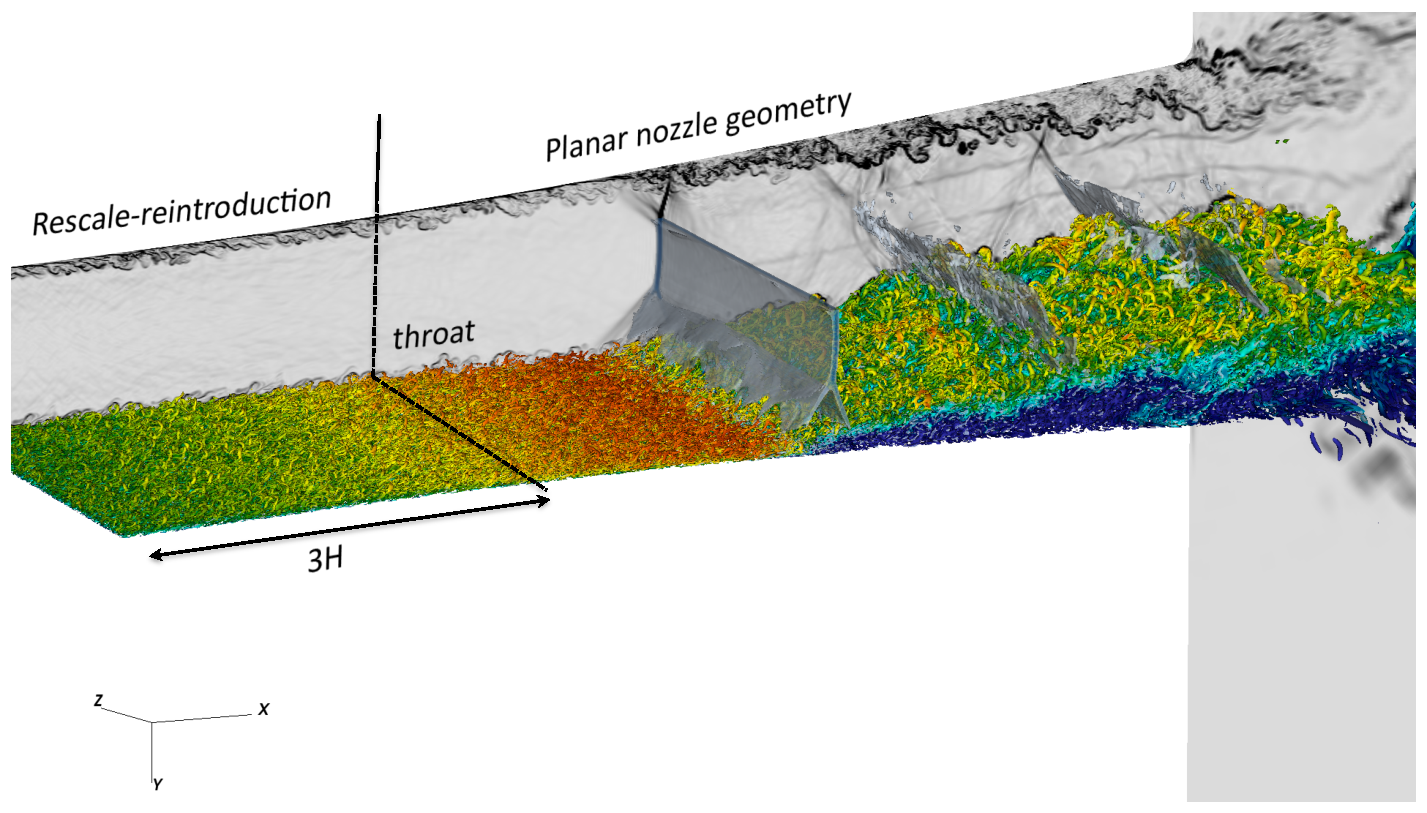
\includegraphics[trim = 0in 1.2in 0in 0in, clip, width = 7in]{figs/info_slide2.pdf}
	\caption{Iso-volume of $|| \nabla\rho ||$  shaded by vorticity magnitude with contours of velocity magnitude in back plane. }
 	\label{fig:info_3d}
\end{figure}

\section{Experimental Setup}

\emph{ Papam's setup looked like this.  The several papers studied bla,bla and bla and found bla.... we are modeling case 3 from PoF 2010 because has asymmetries.  We only do one to establish the suitability of LES and res. requirements.  maybe dont need this?}

The particular experimental configuration that the present LES will model was published the Johnsen and Papamoshcou.~{\cite:Papam:10}.  The geometry for the diverging section is fully defined by the given throat height, $H_t$ and area ratio, $A_e/A_t$.  The contour of the nozzle is simply the solution to a 4th order polynomial with boundary conditions.  Furthermore, the measure of the nozzle's over-expansion is given by the ratio of driver pressure to ambient pressure, or the nozzle pressure ratio (NPR=$p_{res}/p_0$).  The present LES models case 3 from this experiment with an area ratio of 1.6 and NPR of 1.7.  This configuration had the most experimental data available and also had generated large asymmetries in both the shock structure and the subsequent separated shear layer.  

\begin{figure}[!htb]% order of placement preference: here, top, bottom
	\centering
  	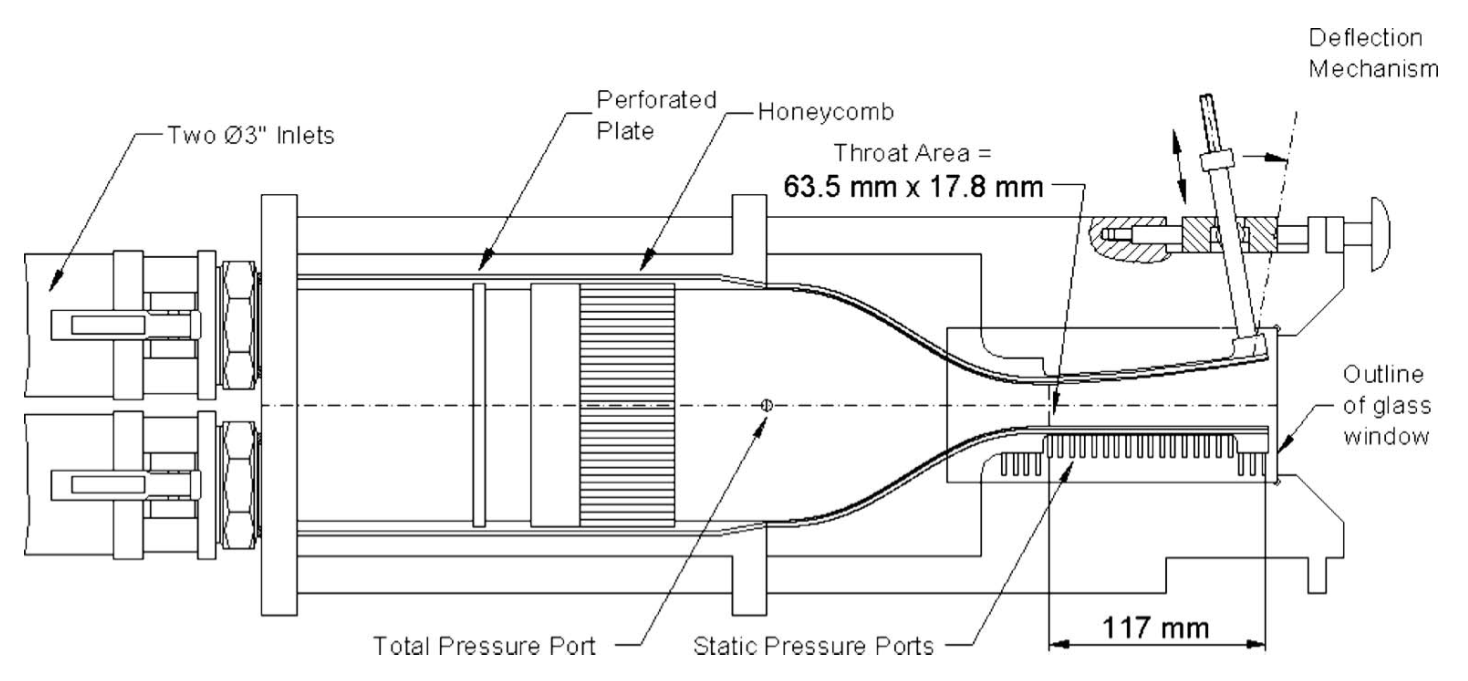
\includegraphics[width = 7in]{../../data/experiment/exp_setup.png}
	\caption{Experimental setup~{\cite:Papam:10} showing the converging and diverging section of the nozzle.  The present LES only explicitly models the diverging section and uses recycled turbulence and the quasi-1D equations to model converging portion. }
 	\label{fig:info_3d}
\end{figure}


\section{Results}

\emph{ We compare results from exp. and highlight the key feature of this complex flow.  We verify incoming BL is wall resolved and converged for the 3 levels of refinement.  
\\  - Mean pressure profile (discuss modeling approach for converging section)
\\  - Mean U and rms profiles.... ( we are capturing the pertinent  length scales well.- higher Re, higher $\delta$ than exp. Also give $Re_\tau$ and $Re_\theta$ of sim.  More modeling assumptions)
\\  - Span-wise correlations.... ( Good results, show our periodic domain is large enough that it doesn't effect the averaged results.  Also suggests that the exp AR might be large enough to have a similar span indep. behavior away from the wall.  ?? 
\\  - Plume PSD.- Ah.. quantity that RANS cant touch.... we nail it.  Coarse calc. is doing well at capturing unsteadiness post shock.
\\  - Wall pressure comp. spec.  General trends are captured and we see good agreement with position (X) and frequency range(St).  Emph. the range and inherit cost of calc.
\\  - Show shock position time history... spectra...  Distinguish difference in methods and potential reasons for discrepancies but show we capture the trends well.  
\\  - Flow asymmetries/ shock structure well represented (show $|\nabla\rho|$ vs. Schlieren).
\\  - Comment on shock motion and separation, RSS+FSS and side loads... show side loads for fun.  Some correlation perhaps?
}

The accuracy of our LES calculation must be established before these data can be used to explore the underlying physics.  This accuracy is measured by comparing against experimental data and performing a mesh refinement study.  Data from the mesh refinement study show the incoming turbulent boundary layer is being captured well.  The periodic span-wise direction, although not truly periodic in the experiment, is sufficiently large for flow structures to be independent of the periodic boundary.  Furthermore, our LES calculations show excellent agreement with both the mean and time dependent quantities from the experiment.  The aforementioned results are shown here to establish the fidelity of our LES database.

Preliminary results from the coarse mesh simulation are presented here.  The computation ran on 256 processors for 2 days which was long enough to wash out initial transients, develop the boundary layer and capture the low frequency oscillations of the shock location.  The coarse calculation attempts to match the particular experimental configuration from Papamoschou et.al.\cite{Papam:09} with a given nozzle pressure ratio ($NPR$) of 1.77 and an area ratio ($A_e/A_t$) of 1.4.  Figure~\ref{fig:info_3d} shows the main features of the over-expanded nozzle experiment.  A normal shock wave is set up inside the nozzle and forces the turbulent boundary layer to separate.  The flow does not reattach and there is a large shear layer downstream as the flow exits into the ambient conditions outside the nozzle.

\subsection{Incoming Turbulent Boundary Layer}

The incoming turbulent boundary layer is well captured by the medium and fine mesh LES.  Viscous length scales near the wall are explicitly modeled with varying grid spacing by the coarse, medium and fine cases.  These spacings are given in viscous wall units in Table~\ref{tbl:mesh} for the different resolution cases.  Mean velocity and RMS profiles (Fig.~\ref{fig:BL_prof}) for the medium and fine case are nearly identical.  The coarse case is shifted upward, indicating a lack of resolution near the wall.  It is also important to note here, the shift upward from the standard the log-law fit($U_{VD}^+ = \log(y^+) / .41+ b $), where $b$ is the intersect.  This is attributed to the substantially large pressure gradient present at the throat.  Spalart~\cite{Spalart:93} investigated the effect of a favorable pressure gradient on the velocity profiles in the boundary layer and found that for a normalized pressure gradient of $\frac{dP}{dx}\frac{\delta}{\tau_w} = -0.3$ there was a shift in $b$ of 20\%.  The pressure gradient at the throat for our current study was calculated to be $\frac{dP}{dx}\frac{\delta}{\tau_w} = -0.7$ and the shift  was 27\%.  The former study by Spalart and the converged LES profiles indicate that the calculation is accuratly capturing the boundary layer and the effect of the favorable pressure gradient.  



\begin{figure}
	\includegraphics[height=2.75in]{../../figs/mean.pdf}
	\includegraphics[height=2.75in]{../../figs/rms.pdf}
	\caption{(Left) Mean velocity profile (Van Driest transformed) in the wall normal direction ($+$ units) for the coarse (dashed), medium (dashed-dot) and fine (solid) mesh cases at the nozzle throat.  Inner and log-law fits are plotted for reference.  (Right) Diagonal components of the Reynolds stress for the three cases.
	\label{fig:BL_prof}
	}
\end{figure}


\subsection{Mean Pressure Profiles}
The mean pressure profile at the centerline and at the wall compare well to the experimental data.  Upstream on the nozzle throat, centerline pressure does not agree with the experiment.  This is expected, as our approach models the converging section using the quasi-1d flow relations and the method recycling-rescaling for the inflow variables and turbulent boundary layer.  Figure \ref{fig:P_prof} show excellent agreement with the experimental data after the throat ($x=0$) indicating that the modeling of the converging section has a minimal effect on the flow past the throat.


\begin{figure}
	\includegraphics[height=2.75in]{../../figs/Pcenter.pdf}
	\includegraphics[height=2.75in]{../../figs/Pwall.pdf}
	\caption{ Mean pressure profiles for the experiment (circles) and LES (dashed) at the centerline (left) and wall (right). 
	\label{fig:P_prof}
	}
\end{figure}

\begin{figure}
	\includegraphics[height=2.75in]{../../figs/dPdx.pdf}
	\includegraphics[height=2.75in]{../../figs/spalart.pdf}
	\caption{ Normalized wall pressure gradient for the experiment (circles) and the LES (dashed) showing agreement passed the throat and its large favorability.
 	\label{fig:dPdx}
	}
\end{figure}

\begin{figure}
	\begin{centering}
	\includegraphics[height=3.75in]{../../figs/mean_st.pdf}

	\caption{ Mean velocity profiles (Van Driest) at various stations along the length of the nozzle.  The sustained favorable pressure gradient causes a further upward shift in the mean profiles.
 	\label{fig:stations}
	}
	\end{centering}
\end{figure}


\begin{figure}
	\includegraphics[height=2.75in]{../../figs/1dspancorr.pdf}
	\includegraphics[height=2.75in]{../../figs/2dspancorr.pdf}
	\caption{ (Left) Two point auto-correlation for the stream-wise component of velocity vs. distance for a point in the pre-shock boundary layer (solid), post-shock boundary layer (dashed) and large separated shear layer (dashed-dotted).  (Right) Contours of the Taylor microscale for the coarse (top) and medium (bottom) calculations.  Data suggest that the LES has sufficient length in the periodic direction($L_z$) for minimal effect of the periodic boundary condition.
 	\label{fig:span_corr}
	}
\end{figure}

\begin{figure}
	\includegraphics[height=2.75in]{../../figs/PSD_compare.pdf}
	\caption{ Normalized Power Spectral Density (PSD) at a point in the large separated shear layer for the LES (solid) and experiment (circles) vs. Strouhal number.  The LES captures the PSD over a large frequency range extremely well, indicating the method is capturing the significant energy containing scales.
 	\label{fig:PSD_comp}
	}
\end{figure}

\begin{figure}
	\begin{centering}
	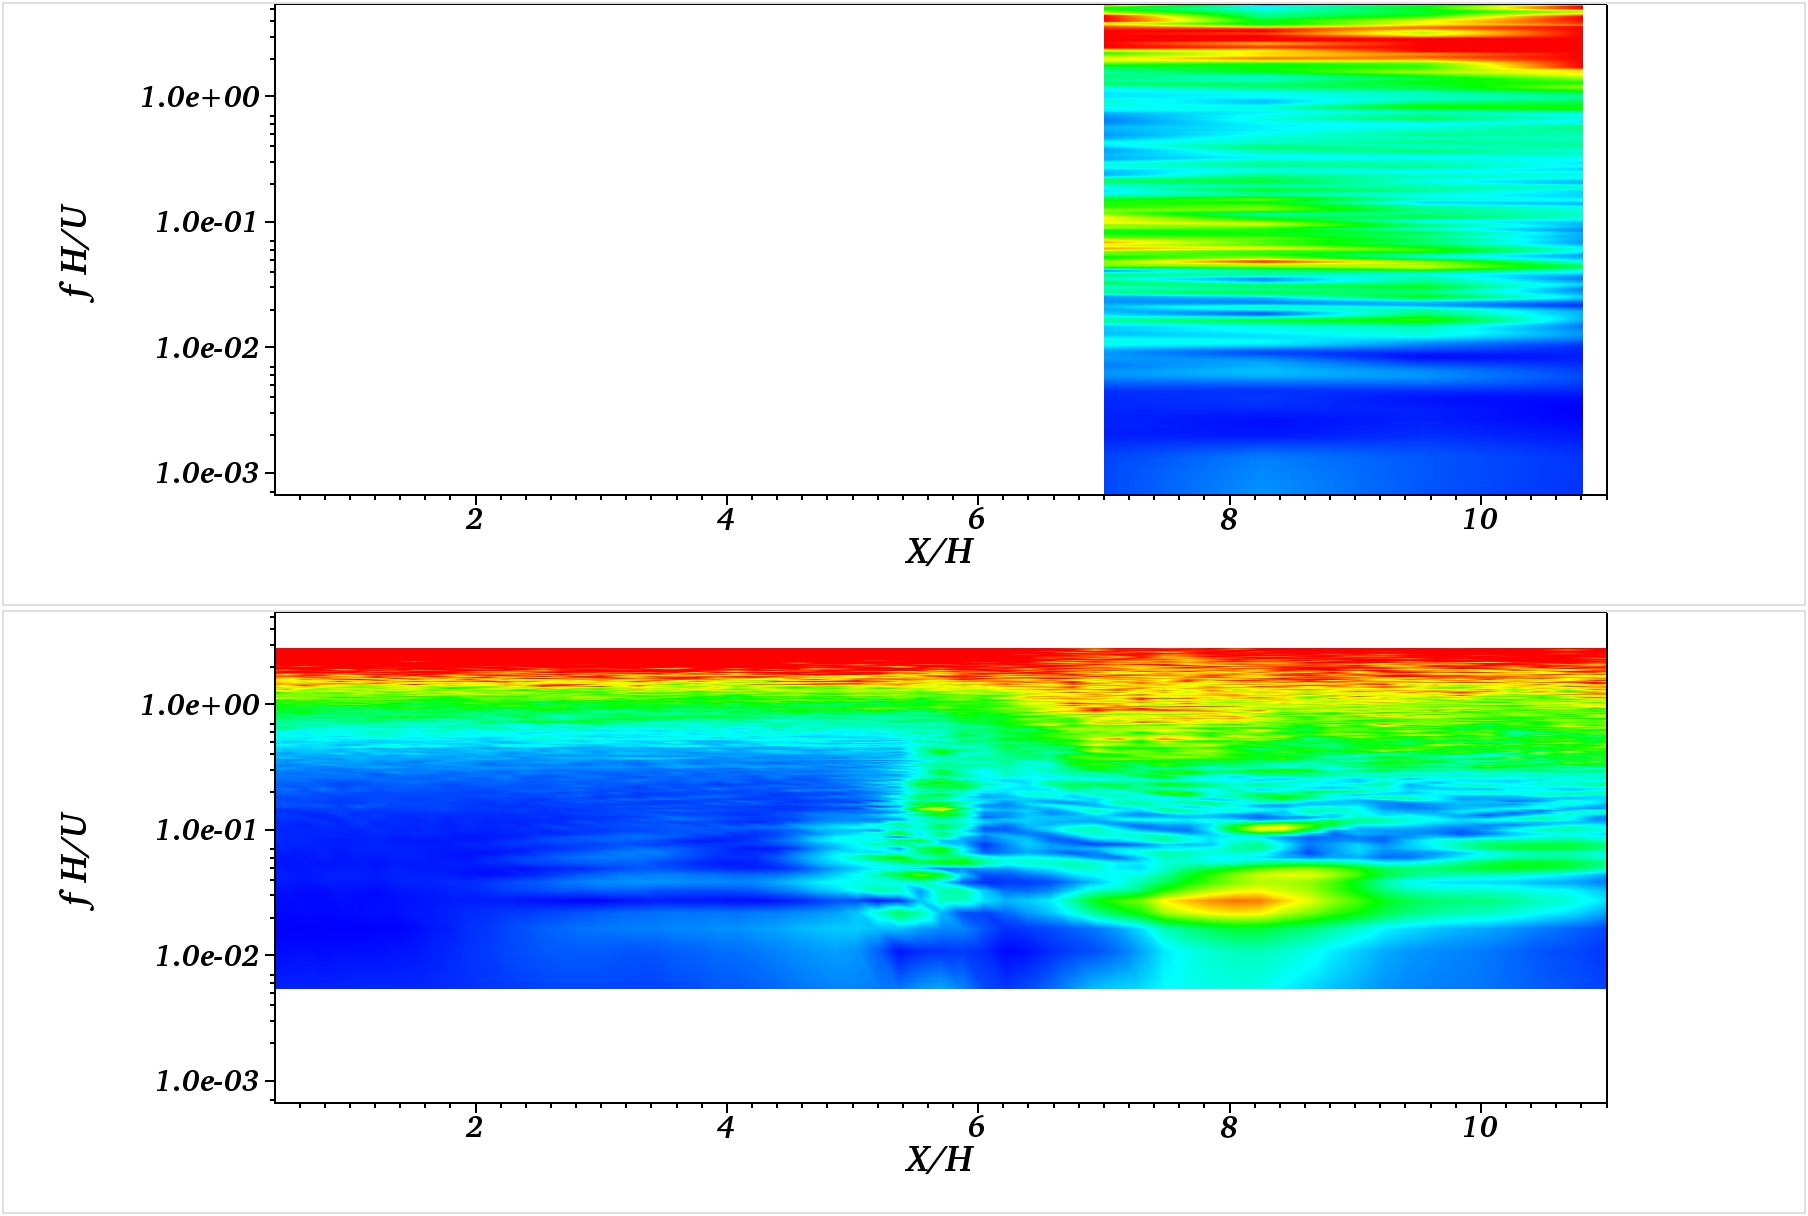
\includegraphics[height=3.75in]{../../figs/XvSt_wall.jpg}
	\caption{ Compensated energy spectra for wall pressure fluctuations normalized such that the integral over frequency at each $x$ location is unity.  Experimental data (top) and LES data (bottom) show both depict the low frequency motion of the shock wave and the high frequency turbulent boundary and shear layer.
 	\label{fig:comp_spectra}
	}
	\end{centering}
\end{figure}

\subsection{Shock Location}
Figure~\ref{fig:schl} shows a comparison between a Schlieren photograph taken from the experiment to results taken from the coarse mesh calculation.  Contours of the density gradient magnitude ($||\nabla\rho|| $) show that the coarse mesh calculation is in good qualitative agreement with the experiment.  The shock location, (which was experimentally reported to oscillate left and right by a distance of +/- $\delta_N$ ) agrees quite well with the experiment.  Furthermore the secondary shocks or the ``aftershocks'' observed in the experiments are captured.  From the experimental Schlieren image, one can clearly observe that there are scales of motion present in the separated shear layer which are not resolved in the coarse mesh calculation, and hence the requirement for subsequent and refined simulations.

\begin{figure}
	\begin{centering}
	\includegraphics[width=6.5in, height=2.5in, keepaspectratio=false]{../../figs/shock_compare.pdf}
	\caption{ Shock wave location time history from the experimental measurements~{\cite:Papam:10} are shown as the original figure in black.  Blue line is data from the LES (coarse mesh) and shows good qualitative agreement.
 	\label{fig:comp_spectra}
	}
	\end{centering}
\end{figure}



\begin{figure}[!htb]% order of placement preference: here, top, bottom
	%\begin{center}
	\centering
	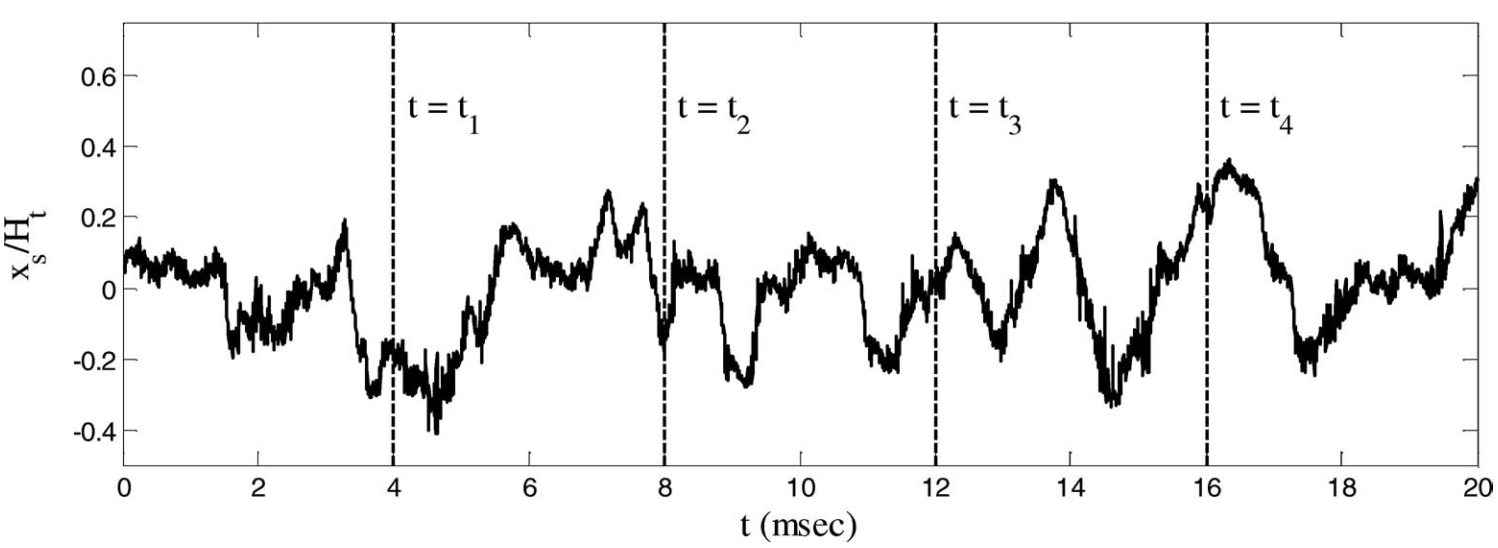
\includegraphics[height=2.5in]{../../figs/shock_history.pdf}
	\includegraphics[height=2.5in]{../../figs/shock_spectra.pdf}
	%\end{center}
 	\caption{Schlieren images from experiment cite{Johnsen:10} (left) and $z$-averaged contours of $||\nabla\rho||$ from the medium mesh LES (right) show excellent qualitative agreement of the shock structure, the separated shear layer and the compression/expansion waves.  }
 	\label{fig:schl}
\end{figure}




\begin{figure}[!htb]% order of placement preference: here, top, bottom
	\begin{center}
	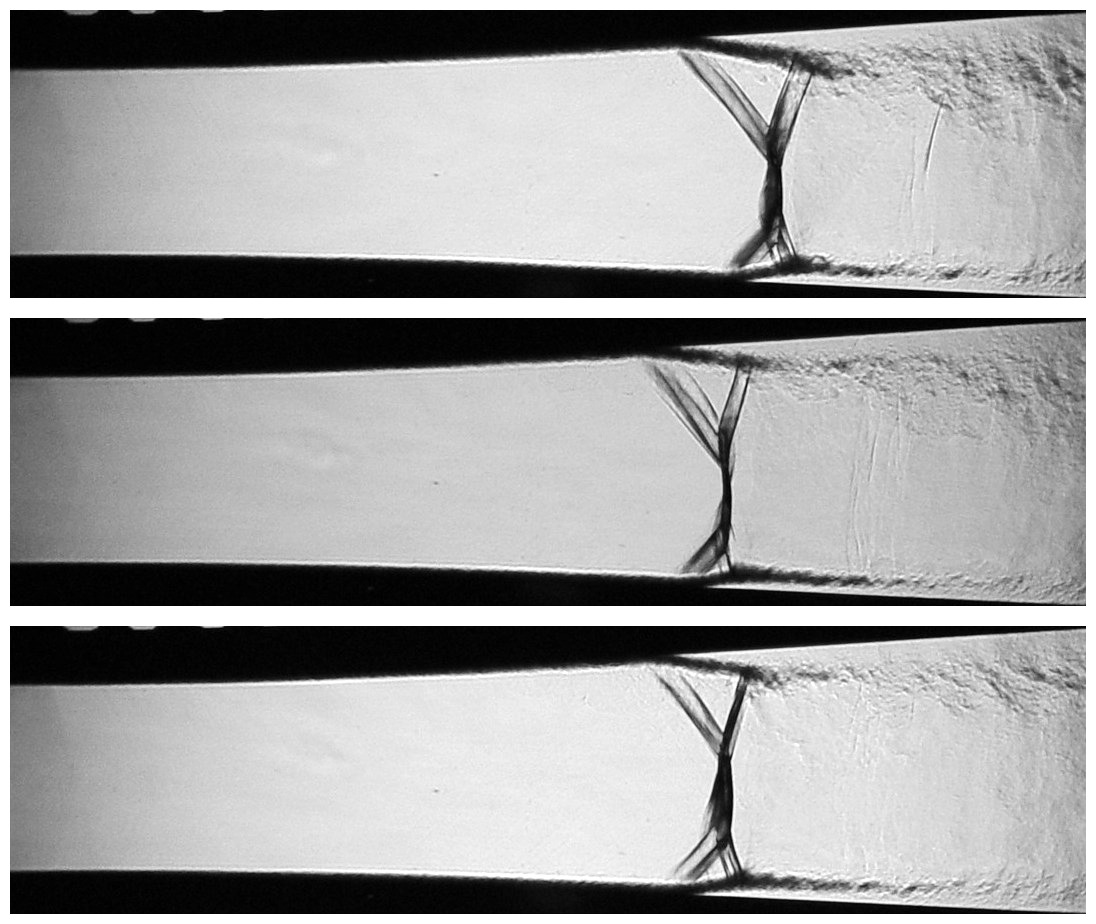
\includegraphics[width=3in]{../../figs/exp_montage.jpg}
	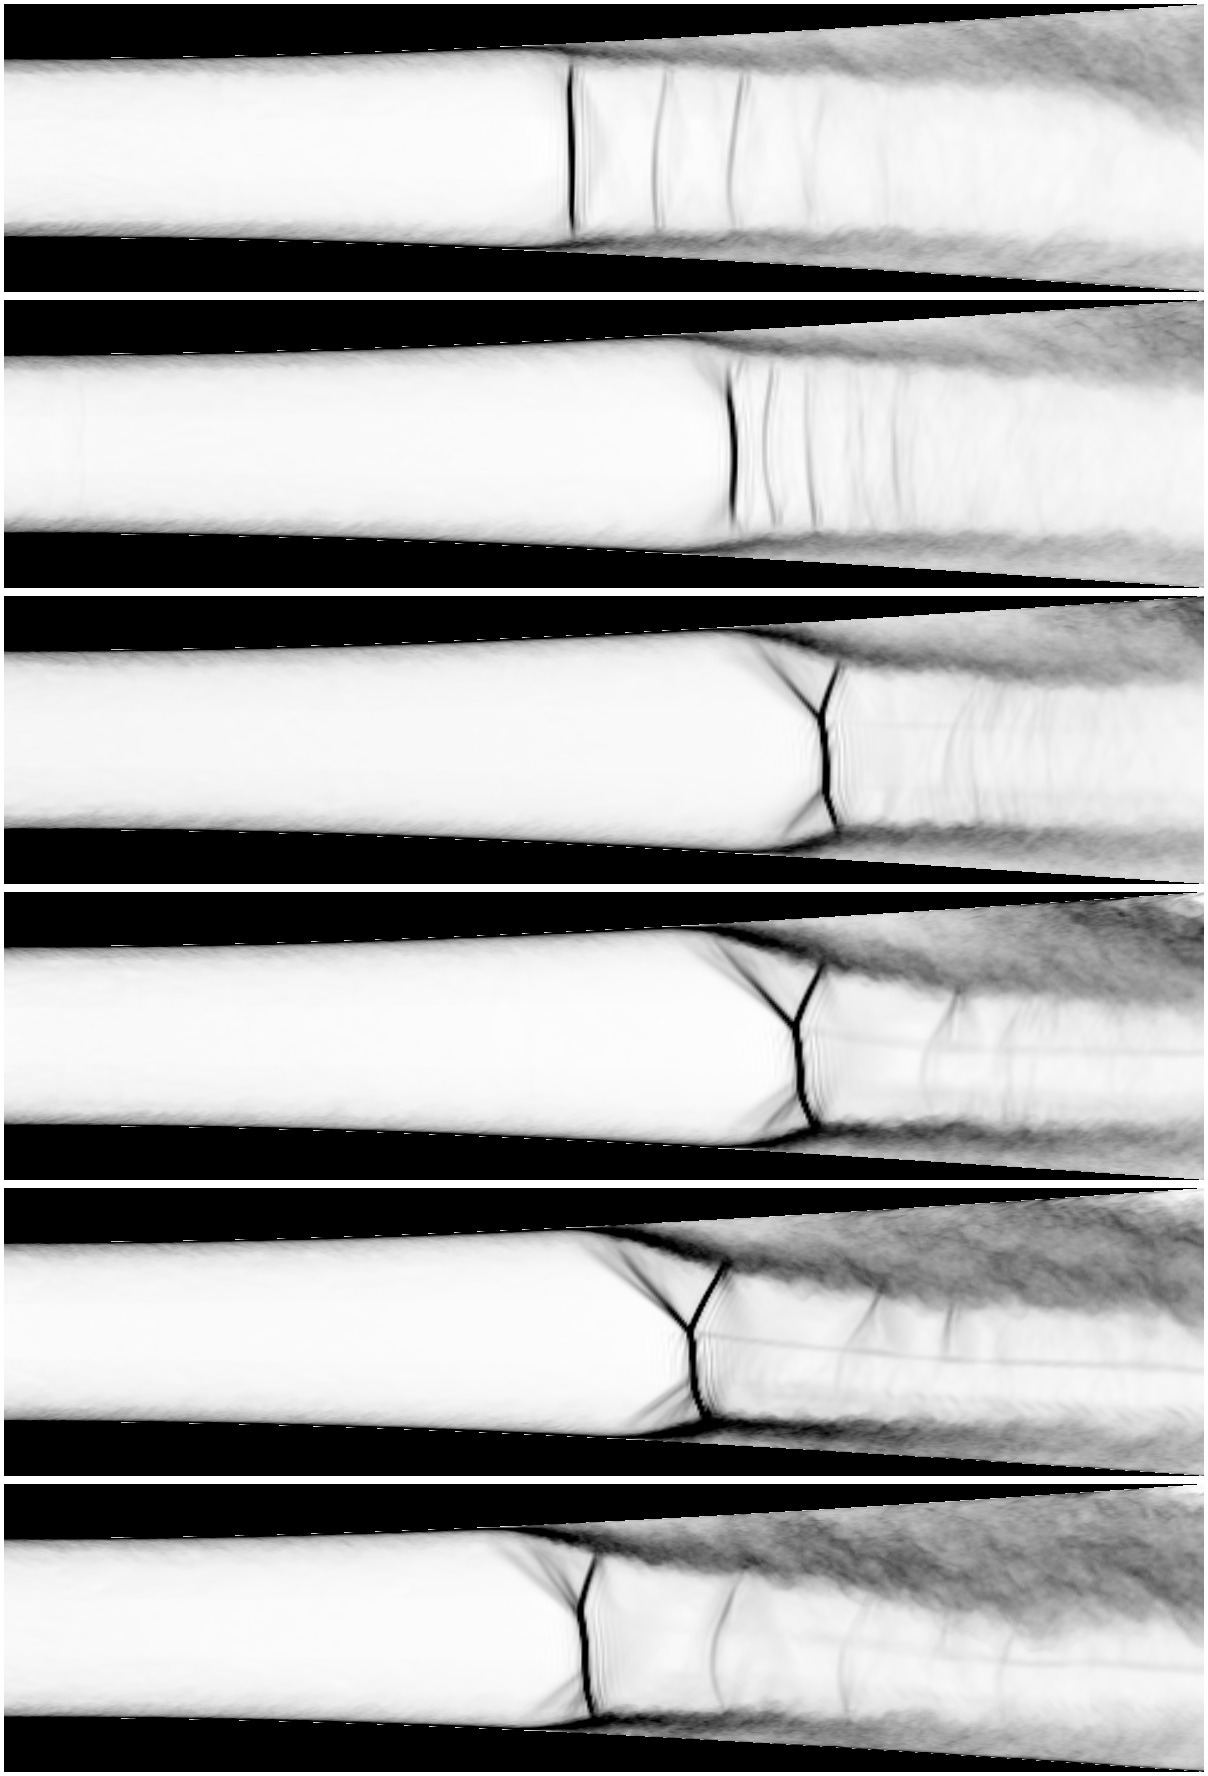
\includegraphics[width=3in]{../../figs/sim_montage.jpg}
	\end{center}
 	\caption{Schlieren images from experiment cite{Johnsen:10} (left) and $z$-averaged contours of $||\nabla\rho||$ from the medium mesh LES (right) show excellent qualitative agreement of the shock structure, the separated shear layer and the compression/expansion waves.  }
 	\label{fig:schl}
\end{figure}


\begin{figure}[!htb]% order of placement preference: here, top, bottom
	\begin{center}
	%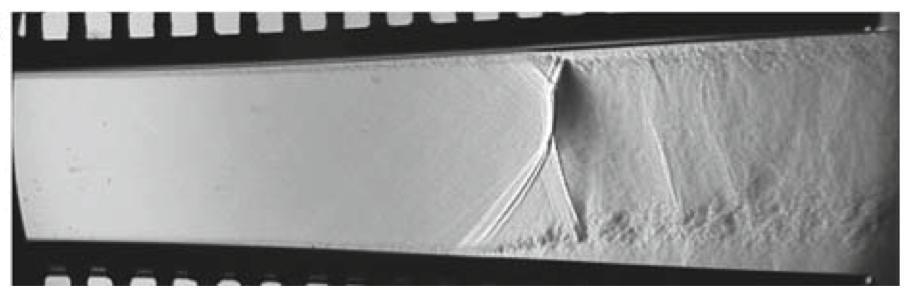
\includegraphics[width=6.1in]{figs/papam_exp.png}
 	%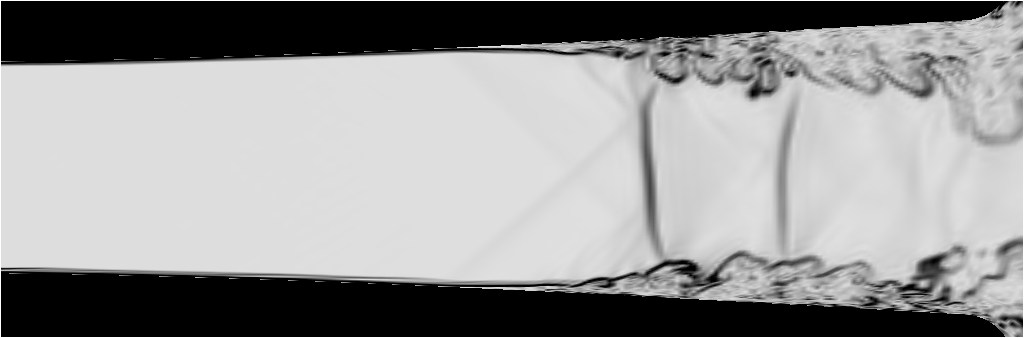
\includegraphics[width=6in]{figs/papam_cLES.png}
	\includegraphics[height=3in, angle=-90]{figs/plume_exp.png}
	\includegraphics[height=3in, angle=-90]{figs/plume_les.png}
	\end{center}
 	\caption{Schlieren images from experiment cite{Johnsen:10} (left) and $z$-averaged contours of $||\nabla\rho||$ from the medium mesh LES (right) show excellent qualitative agreement of the shock structure, the separated shear layer and the compression/expansion waves.  }
 	\label{fig:schl}
\end{figure}


\subsection{Flow asymmetries}
The experimentalists also observed large asymmetries in the shock structure and in the separated shear layer.  Once a preferred side was selected by the flow it was maintained through the duration of the experiment.  This preferred side varied from run to run with a uniformly random distribution.  Again the coarse mesh calculation exhibited identical behavior, selecting a preferred side and maintaining that side for the duration of the simulation.  Both the lambda shock structure and the asymmetric shear layer from the calculation are shown in Figure~\ref{fig:asym}.  We can also observe a rapid change in the turbulent structure of the flow near the wall as the flow passes through the shock wave in Figure~\ref{fig:asymBL}.  The distinct differences in the top and bottom boundary layers illustrate clearly the shock asymmetry present in the flow.


\begin{figure}
  \centering
  
  \subfloat[$\tau=0$]{\includegraphics[width=2in]{figs/medium_figs/medium3dgradRHO_sep_0550.png}}    
  \hspace{0.1in}	            
  \subfloat[$\tau=13.5$]{\includegraphics[width=2in]{figs/medium_figs/medium3dgradRHO_sep_0700.png}}
  \hspace{0.1in}	
  \subfloat[$\tau=27$]{\includegraphics[width=2in]{figs/medium_figs/medium3dgradRHO_sep_0850.png}}
  
  
  \subfloat[$\tau=4.5$]{\includegraphics[width=2in]{figs/medium_figs/medium3dgradRHO_sep_0600.png}}    
  \hspace{0.1in}	            
  \subfloat[$\tau=18$]{\includegraphics[width=2in]{figs/medium_figs/medium3dgradRHO_sep_0750.png}}
  \hspace{0.1in}	
  \subfloat[$\tau=31.5$]{\includegraphics[width=2in]{figs/medium_figs/medium3dgradRHO_sep_0900.png}}
  
  
  \subfloat[$\tau=9$]{\includegraphics[width=2in]{figs/medium_figs/medium3dgradRHO_sep_0650.png}}    
  \hspace{0.1in}	            
  \subfloat[$\tau=22.5$]{\includegraphics[width=2in]{figs/medium_figs/medium3dgradRHO_sep_0800.png}}
  \hspace{0.1in}	
  \subfloat[$\tau=34$]{\includegraphics[width=2in]{figs/medium_figs/medium3dgradRHO_sep_0928.png}}
  
  \caption{Shock wave motion and the corresponding separated shear layer over one low-frequency period.  Contours of $||\nabla\rho||$ are shown in grayscale and colored regions depict negative velocity, where red represents a Mach number of approximately 0.1 and blue is zero.    }
  
  \label{fig:history}
\end{figure}


\begin{figure}
  \centering
  
  \subfloat[$\tau=0$]{\includegraphics[width=2in]{figs/wall/medium3dwall_0550.png}}    
  \hspace{0.1in}	            
  \subfloat[$\tau=13.5$]{\includegraphics[width=2in]{figs/wall/medium3dwall_0700.png}}
  \hspace{0.1in}	
  \subfloat[$\tau=27$]{\includegraphics[width=2in]{figs/wall/medium3dwall_0850.png}}
  
  
  \subfloat[$\tau=4.5$]{\includegraphics[width=2in]{figs/wall/medium3dwall_0600.png}}    
  \hspace{0.1in}	            
  \subfloat[$\tau=18$]{\includegraphics[width=2in]{figs/wall/medium3dwall_0750.png}}
  \hspace{0.1in}	
  \subfloat[$\tau=31.5$]{\includegraphics[width=2in]{figs/wall/medium3dwall_0900.png}}
  
  
  \subfloat[$\tau=9$]{\includegraphics[width=2in]{figs/wall/medium3dwall_0650.png}}    
  \hspace{0.1in}	            
  \subfloat[$\tau=22.5$]{\includegraphics[width=2in]{figs/wall/medium3dwall_0800.png}}
  \hspace{0.1in}	
  \subfloat[$\tau=34$]{\includegraphics[width=2in]{figs/wall/medium3dwall_0928.png}}
  
  \caption{Grayscale is $C_f$ from -0.01 to 0.01 corresponding from black to white.  Colored region depicts $T_{ref}$ (.56,.94) isovolume at .60   }
  
  \label{fig:history}
\end{figure}



%\begin{figure}[!h]% order of placement preference: here, top, bottom
%	\begin{center}
%	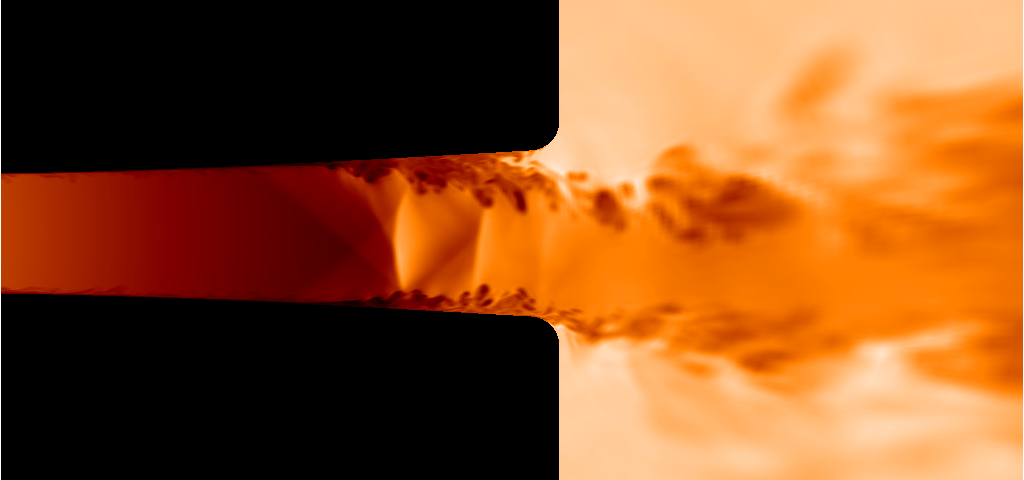
\includegraphics[width=6in]{figs/rho_941s.png}
%	\end{center}
% 	\caption{Contours of density from a 2d slice of the coarse mesh LES showing asymmetries in shock structure and separated shear layer}
% 	\label{fig:asym}
%\end{figure}
%
%\begin{figure}[!h]% order of placement preference: here, top, bottom
%	\begin{center}
%	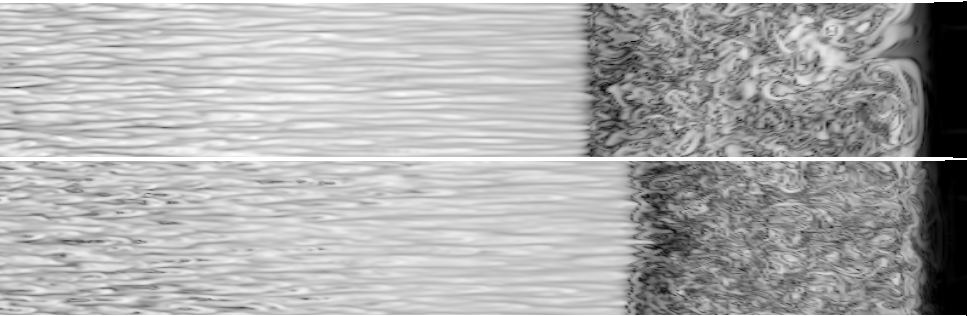
\includegraphics[width=6in]{figs/top_bottom.png}
%	\end{center}
% 	\caption{Contours of density from a 2d slice of the coarse mesh LES at $y^+ \approx 16$ showing asymmetries in shock structure and separated shear layer for top and bottom walls.}
% 	\label{fig:asymBL}
%\end{figure}

\subsection{Outlook for subsequent LES calculations}
The preliminary coarse mesh calculations show surprisingly good results despite the poorly resolved turbulent boundary layer.  It is expected that the medium and fine meshes will produce data which is much richer and complete in the sense that more scales of motion are resolved.  These data sets will be used to compute more quantitative statistics which will be used to compare with the experiment and to advance the understanding of this problem and its complex, underlying physics.  We also plan to conduct a parametric variation with the nozzle pressure ratio to explore the flow regimes observed in the experiments.  

\section{Conclusion}
\emph{We did this LES.  It compared well and we can now look at all kinds of stuff.  New stuff was found ... here we repeat what that was.  }


\section*{Acknowledgments}

This work is supported by the Department of Energy SciDAC2 Grant (Grant DE-FC02-06-ER25787) and the DOE Computational Science Graduate Fellowship.  The authors wish to thank Dr. A. Cook and Dr. W. Cabot for providing the code which was modified for the present study.  

\begin{thebibliography}{10}% maximum number of references (for label width)
 
 \bibitem{Lele:92}
 	S.K. Lele, ``Compact Finite-Difference Schemes With Spectral-Like Resolution,'' \emph{Journal of Computational
	Physics}, Vol. 103, pp. 16-42, 1992.
	
\bibitem{Poinsot:92}
	T.J. Poinsot and S.K. Lele, ``Boundary conditions for direct simulations of compressible viscous flow,'' \emph{Journal of Computational Physics}, 101(1):104-129, 1992

 \bibitem{Cook:07} 
 	A.W. Cook,  ``Artificial Fluid Properties for large-eddy simulation of compressible turbuelnt mixing,'' \emph{Physics of Fluids}, Volume {\bf 19}, 2007.
	
\bibitem{CookCabot:05}
	A.W. Cook and W.H. Cabot, ``Hyperviscosity for shock-turbulence interactions'', \emph{Journal of Computational Physics}, Vol. 203(2):379-385, 2005
 
 \bibitem{Kawai:10}
 	S. Kawai, S. K. Shankar and S. K. Lele, ``Assessment of localized artificial diffusivity scheme for large-eddy simulation of compressible turbulent flows,'' \emph{Journal of Computational Physics}, {\bf 		229} (5), 1739-1762, (2010).
	
 \bibitem{Kawai:10aiaa}
	S. Kawai, S.K. Lele, ``Large-Eddy Simulation of Jet Mixing in Supersonic Cross�ows,'' \emph{AIAA JOURNAL} Vol. 48, No. 9, September 2010.
	
 \bibitem{Touber:09}
 	E. Touber and N.D. Sandham, ``Large-eddy simulation of low-frequency unsteadiness in a turbulent shock-induced separation bubble,'' \emph{Theoretical and Computational Fluid Dynamics} Volume 23, Number 2, 79-107

 \bibitem{Pirozzoli:09}
 	S. Pirozzoli, A. Beer, M. Bernardini and F. Grasso, ``Computational analysis of impinging shock-wave boundary layer interaction under conditions of incipient separation,'' \emph{Shock Waves} Volume 19, Number 6, 487-497

 \bibitem{Kennedy:00}
 	C.A. Kennedy, M.H. Carpenter and R.M. Lewis, ``Low-storage, explicit Runge-Kutta schemes for the compressible Navier-Stokes equations,'' \emph{Appl. Numer. Math.} {\bf 35}, 177 (2000) 
 
 \bibitem{Ostlund:05}
 	J. Ostlund and B. Muhammad-Klingmann,``Supersonic flow separation with application to rocket engine nozzles,'' \emph{Appl. Mech. Rev.} {\bf 58}, 143 (2005).
 
 \bibitem{Papam:10}
 	A.D. Johnson and D. Papamoschou, ``Instability of shock-induced nozzle flow separation,'' \emph{Physics of Fluids}, Volume {\bf 22}, (2010).
	
 \bibitem{Papam:09}
 	D. Papamoschou, A. Zill, A. Johnson, ``Supersonic flow separation in planar nozzles,'' \emph{Shock Waves}, {\bf 19}, 171 (2009).

 \bibitem{Xiao:07}
 	Q. Xiao, H.M. Tsai and D. Papamoschou, ``Numerical investigation of supersonic flow separation,'' \emph{AIAA J.} {\bf 45}, 532 (2007).
	
 \bibitem{Papam:06}
 	D. Papamoschou and A. Johnson, ``Unsteady phenomena in supersonic nozzle flow separation,'' \emph{AIAA J.} 2006-3360, (2006).
	
 \bibitem{Bourgoing:05}
 	A. Bourgoing and Ph. Reijasse, ``Experimental analysis of unsteady separated flows in a super-sonic planar nozzle,'' \emph{Shock Waves} {\bf 14}, 251 (2005).
	
 \bibitem{Dussauge:09}
 	S. Piponniau, J.P. Dussauge, J.F. Debieve and P. Dupont, ``A simple model for low-frequecy unsteadiness in shock induced separation,'' \emph{J. Fluid Mech.}, vol. {\bf 629}, pp. 87-108 (2009).
	
 \bibitem{Lund:98}
 	T.S. Lund, X. Wu, and K.D. Squires, ``Generation of Turbulent Inflow Data for Spatially-Developing Boundary Layer 
Simulations,'' \emph{Journal of Computational Physics}, Vol. 140, No. 2, 1998, pp. 233-258.

 \bibitem{Morgan:10a} 
 	B. Morgan, J. Larsson, S. Kawai and S.K. Lele, ``An Improved Method for Prescribing Turbulent Boundary Layer 
Inflow'', \emph{AIAA Journal}, submitted for publication, June, 2010.

 \bibitem{Morgan:10b} 
 	B. Morgan,S. Kawai and S.K. Lele, ``Large-Eddy Simulation of an Oblique Shock Impinging on a 
Turbulent Boundary Layer'', \emph{AIAA Journal}, 2010-4467, 2010.
 	
 \bibitem{Bookey:05}
 	P.B. Bookey, C. Wyckham, A.J. Smits, and M.P. Martin, ``New Experimental Data of STBLI at DNS/LES Accessible 
Reynolds Numbers,''  AIAA Paper 2005-309, Jan. 2005.

\bibitem{Spalart:93}
	P. Spalart and J. Watmuff, ``Experimental and numerical study of a turbulent boundary layer with pressure gradients,'' \emph{J. Fluid Mech.},
vol. {\bf 249}, pp. 337-371 (1993)	

 
	
\end{thebibliography}

\end{document}

% - Release $Name:  $ -
